\chapter{Przegląd literatury}

\section{Cele badania przestrzeni rozwiązań}
Analiza przestrzeni rozwiązań pozwala na lepsze poznanie niektórych cech problemu, a także zbadanie, w jakim stopniu cechy te zależne są od
rodzaju badanej instancji. Przedmiotem badań z tej dziedziny najczęściej są znane problemy NP-trudne, takie jak problem komiwojażera czy problem kwadratowego przydziału.
Jednym z proponowanych zastosowań analizy przestrzeni rozwiązań jest wykorzystanie jej do wyboru najlepszego algorytmu heurystycznego
dla danej instancji problemu. W pracy \textit{Local Optima Networks in Solving Algorithm Selection Problem for TSP}\cite{DBLP:conf/depcos/BozejkoGNAB18}
sieci optimów lokalnych wygenerowane na podstawie próbkowania przestrzeni rozwiązań wykorzystano do nauczenia modeli regresji, których zadaniem było
przewidzenie, który algorytm heurystyczny da lepsze wyniki dla danej instancji problemu.
Badanie wykazało, że analiza przestrzeni rozwiązań może zostać z powodzeniem wykorzystana w tym celu.
Problemem pozostaje natomiast długi czas trwania próbkowania przestrzeni, zwykle dłuższy niż czas działania samego algorytmu heurystycznego.
W pracy \textit{Mapping the global structure of TSP Fitness landscapes}\cite{DBLP:journals/heuristics/OchoaV18} zbadano przestrzeń rozwiązań
dla różnych instancji problemu komiwojażera. Zauważono, że instancje wygenerowane losowo zwykle mają mniejszą neutralność i mniej globalnych optimów od
instancji rzeczywistych. Zaobserwowano również, że sposób rozłożenia miast (w klastrach, równomierny) wpływa na wzajemną korelację wartości różnych miar.

W ostatnich latach w podobny sposób przeprowadzono analizy przestrzeni konfiguracji wieloparametrowych algorytmów optymalizacyjnych.
W pracy \textit{Understanding Parameter Spaces using Local Optima Networks: A Case Study on Particle Swarm Optimization}\cite{DBLP:conf/gecco/CleghornO21}
wykorzystano sieci lokalnych optimów, oraz pochodne struktury CMLON do analizy i wizualizacji przestrzeni parametrów algorytmu roju cząstek.
Analiza wykazała istnienie dużej ilości lokalnych optimów, niską neutralność, oraz istnienie wielu ścieków (ang sinks) nie znajdujących się w optimum globalnym,
Sugeruje to, że naiwne metody dobierania parametrów mogą łatwo doprowadzić do suboptymalnej konfiguracji i w efekcie nie otrzymania najlepszych wyników.
Podobne badanie wykonano dla przestrzeni parametrów procesu AutoML w pracy \textit{Understanding AutoML Search Spaces with Local Optima Networks}\cite{DBLP:conf/gecco/TeixeiraP22}.
AutoML jest procesem automatyzacji konfiguracji procesów (ang. pipelines) uczenia maszynowego obejmującym m. in. wybór zastosowanego przetwarzania wstępnego,
właściwego algorytmu uczenia, oraz jego hiperparametrów. W pracy zbadano przestrzeń konfiguracji AutoML dla zadania klasyfikacji.
Jako funkcję celu przyjęto uśrednioną wartość metryki F-score dla danej konfiguracji procesu.
Wartości F-score uzyskano poprzez przetestowanie procesu na kilku zbiorach danych.
Dla każdej z badanych przestrzeni konfiguracji utworzono trzy sieci LON. Każda z sieci była oparta o inny model krawędzi.
Przeszukano wszystkie możliwe rozwiązania, ale ze względu na złożoność obliczeniową sieć LON budowano poprzez przeglądanie
ograniczonego sąsiedztwa każdego z wierzchołków. Badanie wykonano dla kilku wielkości sąsiedztwa - 20, 30, 50 i 100 sąsiadów.
Zauważono wpływ modelu krawędzi na powstałą sieć - w sieciach z krawędziami typu basin-transition nie zauważono obecności ścieków,
natomiast istniało wiele źródeł. Sieci oparte o escape edges miały z kolei dużo ścieków i mało źródeł.
W przypadku perturbation edges w sieci nie było ścieków ani źródeł niezależnie od rozmiaru sąsiedztwa.
Zauważono, że w badanych przypadkach optima globalne skupiały się w pewnym rejonie przestrzeni rozwiązań, w niewielkiej od siebie odległości.
Nie były rozłożone równomiernie. Sugeruje to, że w problemie konfiguracji procesu uczenia maszynowego, najlepsze ze wszystkich możliwych
konfiguracji niewiele się od siebie różnią.


\section{Próbkowanie przestrzeni rozwiązań}
Przegląd zupełny przestrzeni rozwiązań problemów trudnych obliczeniowo jest w praktyce niemożliwy, poza bardzo małymi instancjami problemu.
Z tego powodu analizę przestrzeni rozwiązań przeprowadza się na części przestrzeni zbadanej w procesie próbkowania. \\
W tym miejscu pojawiają się pytanie: w jaki sposób próbkować przestrzeń, aby cechy jej zbadanego fragmentu
jak najlepiej odzwierciedlały cechy całej przestrzeni?

Próbkowanie przestrzeni rozwiązań wykonuje się zwykle poprzez zastosowanie pewnej odmiany iteracyjnego przeszukiwania lokalnego
(ang. ILS - Iterated Local Search),
a wyniki zapisuje się w postaci sieci optimów lokalnych.
Najczęściej stosowane algorytmy próbkowania oparte o ILS można podzielić na trzy kategorie:
Próbkowanie dwufazowe, \textit{Markov-chain} oraz \textit{Snowball}.

Próbkowanie dwufazowe składa się z dwóch faz - najpierw próbkowane są wierzchołki poprzez zastosowanie metody iteracyjnego przeszukiwania lokalnego\cite{DBLP:journals/corr/OchoaVDT14}.
Metoda ta polega na generowaniu losowego rozwiązania, a następnie wykorzystaniu algorytmu optymalizacji lokalnej do znalezienia najbliższego
lokalnego optimum. Następuje po tym wylosowanie nowego punktu i powtórzenie procedury.
Druga faza to faza próbkowania krawędzi, polegająca na poddaniu znalezionych wcześniej rozwiązań operacji perturbacji, a następnie wykonaniu optymalizacji
lokalnej. Jeśli otrzymane w ten sposób rozwiązanie jest innym lokalnym optimum znajdującym się w zbiorze wierzchołków, to dodawana jest odpowiednia krawędź.
Metoda ta po raz pierwszy została zaprezentowana w pracy\cite{10.1145/2576768.2598275} do analizy problemu kwadratowego przypisania.
W pracy\cite{DBLP:conf/depcos/BozejkoGNAB18} algorytm oparty o tę samą metodę został wykorzystany do badania przestrzeni problemu komiwojażera.
Zastosowana tam odmiana wykorzystuje algorytm 2-opt do optymalizacji lokalnej i procedurę \textit{2-exchange} jako operację perturbacji.

Metoda \textit{Markov-chain} została po raz pierwszy zaprezentowana w pracy \cite{markovchain}.
Zaczyna się od wybrania losowego rozwiązania i jego optymalizacji. Następnie otrzymane optimum lokalne zostaje poddane operacji perturbacji
i otrzymywane w ten sposób rozwiązanie staje się nowym punktem startowym. Procedura jest powtarzana przez określoną liczbę iteracji, z każdą iteracją
zapisywane są informacje o nowych krawędziach i wierzchołkach.
Metoda została wykorzystana w pracy\cite{DBLP:journals/heuristics/OchoaV18} do badania przestrzeni problemu komiwojażera.
Do optymalizacji lokalnej wykorzystany został algorytm Lin-Kerninghan, a jako operacja perturbacji procedura \textit{Double-bridge}.

Metoda \textit{Snowball} składa się z dwóch etapów wykonywanych naprzemiennie. Pierwszy polega na kilkukrotnym poddaniu rozwiązania początkowego perturbacji
w celu uzyskania sąsiednich rozwiązań, a następnie ich optymalizacji. Procedura jest rekurencyjnie powtarzana dla znalezionych w ten sposób lokalnych optimów
aż do osiągnięcia pewnej z góry ustalonej głębokości. Jedno z lokalnych optimów sąsiadujących z rozwiązaniem początkowym zostaje wybrane jako rozwiązanie początkowe kolejnej iteracji.
Dodatkowo w pamięci przechowywana jest lista rozwiązań początkowych - jeśli rozwiązanie już się w nim znajduje, to nie może być wybrane ponownie.
Jeśli nie istnieje rozwiązanie sąsiednie spełniające ten warunek, za kolejne rozwiązanie początkowe przyjmowane jest lokalne optimum otrzymane z optymalizacji rozwiązania losowego.
Algorytm \textit{Snowball} wywodzi się z technik wykorzystywanych w badaniach z dziedziny socjologii, a w kontekście badania przestrzeni rozwiązań
problemów optymalizacyjnych został zaprezentowany po raz pierwszy w pracy \cite{DBLP:conf/ppsn/VerelDOT18}.

W pracy\cite{DBLP:conf/evoW/ThomsonOV19} zostało przeprowadzone statystyczne porównanie algorytmów próbkowania \textit{Snowball}
oraz \textit{Markov-chain}. Eksperyment polegał na spróbkowaniu 30 instancji problemu kwadratowego przypisania, a następnie użyciu zebranych danych
do stworzenia modeli regresji przewidujących jakość rozwiązań, które zostaną uzyskane przez algorytm optymalizacji uruchomiony na instancji.
Wybranymi algorytmami heurystycznymi były \textit{Robust Taboo Search} Taillarda oraz \textit{Improved ILS} Stützla.
Z zebranych danych utworzono grafy LON i zbadano takie właściwości, jak średnia wartość funkcji celu, średni stopień wychodzący
wierzchołków w grafie, promień grafu, liczba lokalnych optimów i liczba krawędzi.
Stworzono modele regresji typu liniowego oraz lasu losowego. Obliczono wartości korelacji pomiędzy właściwościami przestrzeni rozwiązań
a jakością rozwiązań zwracanych przez algorytmy optymalizacji.
Badania wykazały, że dane pozyskane z próbkowania \textit{Markov-chain} były w większym stopniu skorelowane z jakością rozwiązań algorytmów
optymalizacji, a modele regresji utworzone na ich podstawie dokonywały lepszej predykcji niż te utworzone na podstawie danych ze \textit{Snowball}.
Z kolei \textit{Snowball} okazał się bardziej przewidywalny i łatwiejszy w doborze parametrów.

Podobne badanie przeprowadzono w pracy\cite{DBLP:journals/ec/ThomsonOVV20}, tym razem na większej liczbie instancji
- 124 instancji ze zbioru QAPLIB i dodatkowych 60 instancji o rozmiarze N=11.
Dla tych dodatkowych instancji, oprócz próbkowania wykonano również przegląd zupełny.
Zauważono, że algorytm \textit{Snowball} produkuje gęstszą sieć od algorytmu \textit{Markov-chain}.
Dostrzeżono wadę algorytmu \textit{Snowball} - duży wpływ parametrów próbkowania na wartości metryk opartych o gęstość
i wzory połączeń krawędzi, oraz metryk opisujących struktury lejowe.
Stworzono modele regresji przewidujące jakość rozwiązań generowanych przez heurystyki \textit{Taboo Search} i ILS.
Model przewidujący odpowiedź ILS oparty o dane z algorytmu Snowball był nieco lepszy od modelu opartego o dane z algorytmu ILS.
Między predykcjami modeli przewidujących odpowiedź algorytmu TS nie było znaczącej różnicy.
Wśród wszystkich czterech testowanych modeli cechą przestrzeni będącą najlepszym predyktorem okazała się średnia wartość
funkcji dopasowania (ang. mean fitness).
Porównanie spróbkowanych sieci LON małych instancji z sieciami uzyskanymi
poprzez przegląd zupełny wykazało, że zarówno \textit{Markov-chain} jak i \textit{Snowball}
dobrze aproksymują liczbę wierzchołków i krawędzi w sieci.
\textit{Snowball} odnalazł prawie wszystkie optima lokalne obecne w pełnej sieci.
\textit{Markov-chain} znalazł ich mniej, ale nadal dawał zadowalający wynik.

Z innych prac z dziedziny warto wymienić\cite{DBLP:journals/corr/abs-1207-4455}, w którym porównano algorytmy wstępujące (hillclimb)
typu \textit{best-improvement} i \textit{first-improvement} w próbkowaniu przestrzeni NK.
Wykorzystanie algorytmu typu \textit{first-improvement} prowadziło do powstania gęstszej, bardziej kompletnej sieci optimów lokalnych.
Pętle obecne w sieci miały mniejszą wagę w przypadku algorytmu \textit{first-improvement} co sugeruje, że łatwiej wychodzi z optimum lokalnego.
Dodatkową zaletą tego algorytmu jest krótszy czas wykonywania, spowodowany brakiem konieczności przeglądania za każdym razem całego sąsiedztwa
rozwiązania początkowego.

Z kolei w pracy\cite{DBLP:conf/evoW/McMenemyVO18} zbadano wpływ siły perturbacji (stopnia, w jakim operacja perturbacji zmienia rozwiązanie początkowe)
na właściwości spróbkowanej przestrzeni. Wybranym algorytmem próbkującym był algorytm typu \textit{Markov-chain} pochodzący z artykułu\cite{DBLP:journals/heuristics/OchoaV18}.
Operacją perturbacji tego algorytmu jest procedura double-bridge. Badania przeprowadzono na 180 instancjach o znanych rozwiązaniach optymalnych,
uzyskanych przy pomocy generatora DIMACS TSP . Celem było znalezienie takiego parametru k - siły perturbacji - aby uzyskać jak największy wskaźnik sukcesu.
Za wskaźnik sukcesu przyjęto stosunek liczby przebiegów algorytmu, które znalazły globalne optimum do wszystkich przebiegów.
Nie znaleziono uniwersalnej najlepszej wartości parametru k. Zauważono jednak, że niższa siła perturbacji sprawdzała się dla instancji,
w których miasta rozmieszczone są w klastrach. Dla instancji z miastami rozmieszczonymi równomiernie zwiększanie wartości k powodowało
zmniejszenie ilości suboptymalnych lejów w przestrzeni.
Zaobserwowano również, że instancje z miastami ułożonymi w klastrach były generalnie prostsze do rozwiązania, niż instancje z rozkładem równomiernym,
a także, że rozkład optimów lokalnych w przestrzeni rozwiązań ma większy wpływ na trudność znalezienia optymalnego rozwiązania dla
danej instancji, niż ich ilość.

\section{O przestrzeni rozwiązań}
Przestrzeń rozwiązań (Krajobraz adaptacyjny, ang. Fitness Landscape) jest pojęciem wywodzącym się z biologii ewolucyjnej.
W kontekście biologicznym jest to model opisujący relację między genotypem i fenotypem organizmów, a ich przystosowaniem (ang. fitness),
które jest miarą opisującą sukces reprodukcyjny\cite{FRAGATA201969}.

W kontekście optymalizacji Fitness landscape to trójka $(S, V, f)$, gdzie:
\begin{itemize}
      \item $S$ jest zbiorem wszystkich możliwych rozwiązań - przestrzenią przeszukiwania,
      \item $V$ jest funkcją przypisującą każdemu rozwiązaniu $s\in{S}$ zbiór sąsiadów $V(s)$,
      \item $f$ jest funkcją $f:S \rightarrow \mathbb{R}$ przypisującą danemu rozwiązaniu wartość przystosowania
            - zwykle jest to wartość funkcji celu dla danego rozwiązania.
\end{itemize}

\subsection{Sieć optimów lokalnych}
Sieć optimów lokalnych(ang. Local Optima Network, LON) jest konstruktem zaprezentowanym po raz pierwszy w artykule\cite{PhysRevE.78.066114},
i rozwiniętym w pracy\cite{DBLP:journals/corr/OchoaVDT14}.

Jest to graf $G = (N, E)$ przedstawiający występujące w przestrzeni rozwiązań optima lokalne (zbiór wierzchołków $N$)
i relacje między nimi (zbiór krawędzi $E$).

\subsection{Wierzchołki}
Wierzchołki w sieci optimów lokalnych reprezentują optima lokalne w przestrzeni rozwiązań.
Do optimów zaliczamy minima i maksima; w problemach optymalizacyjnych zazwyczaj poszukujemy tych pierwszych.
Minimum lokalne to takie rozwiązanie $s$, w którego sąsiedztwie $V(s)$ nie znajduje się żadne rozwiązanie $x$, dla którego $f(x) < f(s)$.
Każde rozwiązanie w przestrzeni rozwiązań można przyporządkować do pewnego lokalnego minimum.
Aby znaleźć lokalne minimum $n \in{N}$, do którego "prowadzi" dane rozwiązanie $s\in{S}$, wykonuje się lokalną optymalizację
z tym rozwiązaniem przyjętym jako punkt startowy.
W dalszej części pracy takie przyporządkowanie będzie oznaczane jako $h(s) \rightarrow n\in{N}$.
Wierzchołkom w sieci LON można przypisać wagę równą wartości funkcji celu w danym optimum lokalnym.

\subsection{Krawędzie}
Krawędzie w sieci lokalnych optimów mogą być zdefiniowane na jeden z kilku sposobów.
W literaturze\cite{DBLP:journals/corr/OchoaVDT14}\cite{DBLP:conf/gecco/TeixeiraP22} zostały opisane trzy różne modele:
\textit{basin-transition}, \textit{escape edges} i \textit{perturbation edges}.

\subsubsection{Basin-transition}
Basen przyciągania optimum lokalnego $n$ jest zdefiniowany jako zbiór:
$$b_i = \{s\in{S} \mid h(s) = n\}$$
Rozmiarem basenu jest liczność tego zbioru oznaczana jako $|b_i|$.
Dla każdej pary rozwiązań w przestrzeni można obliczyć prawdopodobieństwo przejścia z jednego rozwiązania do drugiego $p(s \rightarrow s')$.
Dla rozwiązań reprezentowanych permutacją o długości M, prawdopodobieństwo takie wynosi:
$$p(s \rightarrow s') = \frac{1}{M(M-1)/2}, \quad \text{jeżeli} \quad s'\in{V(s)},$$
$$p(s \rightarrow s') = 0, \quad \text{jeżeli} \quad s'\notin{V(s)},$$

Mając informacje o prawdopodobieństwach przejścia między poszczególnymi rozwiązaniami można obliczyć prawdopodobieństwo
przejścia od rozwiązania $s$ do dowolnego rozwiązania należącego do basenu $b_j$:
$$p(s \rightarrow b_j) = \sum_{s'\in{b_j}} p(s \rightarrow s')$$

Całkowite prawdopodobieństwo przejścia z basenu jednego optimum lokalnego do drugiego wynosi więc:
$$p(b_i \rightarrow b_j) = \frac{1}{|b_i|} \cdot \sum_{s\in{b_i}} p(s \rightarrow b_j)$$

To całkowite prawdopodobieństwo stanowi wagę krawędzi w grafie.

Krawędzie typu \textit{basin-transition} tworzą gęstszą sieć od krawędzi typu \textit{escape edges}.

\subsubsection*{Escape Edges}
Escape Edges zdefiniowane są przy pomocy funkcji dystansu $d$ zwracającej najmniejszą odległość między dwoma rozwiązaniami,
oraz liczby całkowitej D.
Krawędź $e_{ij}$ między lokalnymi optimami $n_i$ i $n_j$ istnieje, jeśli istnieje rozwiązanie $s$ takie, że:
\begin{equation}
      \label{eq:escape_edge_cond}
      d(s, n_i) \leq D \land h(s)=n_j
\end{equation}
Wagą takiej krawędzi jest ilość rozwiązań spełniających powyższy warunek.

\subsubsection{Perturbation edges}
W tym modelu wagę krawędzi pomiędzy lokalnymi optimami $n_i$ i $n_j$ uzyskuje się poprzez kilkukrotne wykonanie
operacji perturbacji(mutacji) na $n_i$, a następnie optymalizacji lokalnej otrzymanego rozwiązania.
Liczba przypadków, w których po optymalizacji otrzymujemy rozwiązanie $n_j$ podzielona przez liczbę prób stanowi wagę krawędzi.

$$
      w_{ij} = \frac{ |\{opt(mut(n_i)) = n_j\}| }{trials}
$$

TODO: czy zapis jest poprawny $\land$ ?

\subsection{Struktury lejowe}
W sieci optimów lokalnych możemy wyróżnić sekwencje złożone z optimów lokalnych, których wartość przystosowania jest niemalejąca.
Sekwencje te zwane są sekwencjami monotonicznymi\cite{DBLP:journals/heuristics/OchoaV18}.
Sekwencje monotoniczne zmierzające do tego samego ścieku (ang. sink, wierzchołek bez krawędzi wychodzących)
tworzy strukturę zwaną lejem. Wspomniany ściek stanowi spód leja (ang. funnel bottom), a liczba wierzchołków zawartych w tej strukturze określa jej rozmiar.
Ponadto w przestrzeni rozwiązań można wyróżnić lej pierwszorzędny(ang. primary funnel), kończący się w globalnym optimum i leje drugorzędne,
kończące się w optimach lokalnych. Jeden wierzchołek w grafie może przynależeć jednocześnie do wielu lejów.

Leje w sieci optimów lokalnych można zidentyfikować poprzez usunięcie z grafu krawędzi prowadzących od lepszych rozwiązań do gorszych,
zidentyfikowanie ścieków, odwrócenie krawędzi i wykonanie przeszukiwania wgłąb lub wszerz w celu odnalezienia wierzchołków należących do leja.
\subsection{Metryki przestrzeni rozwiązań} \label{sec:metrics}

\begin{itemize}
      \item \textbf{num\_sinks} - liczba ścieków. Ściek (ang. sink) jest wierzchołkiem grafu nie posiadającym krawędzi wychodzących.
            Pętle nie są uwzględniane.
      \item \textbf{num\_sources} - liczba źródeł. Źródło (ang. source) jest wierzchołkiem grafu nie posiadającym krawędzi wchodzących.
            Pętle nie są uwzględniane.
      \item \textbf{num\_subsinks} - Liczba wierzchołków, które nie posiadają krawędzi wychodzących do rozwiązań o niższej wartości funkcji celu.
      \item \textbf{edge\_to\_node} - stosunek liczby krawędzi do liczby wierzchołków w grafie.
      \item \textbf{avg\_fitness} - średnia wartość funkcji celu lokalnych optimów w sieci.
      \item \textbf{distLO} - średnia odległość rozwiązań od rozwiązania z najniższą wartością funkcji celu. Odległość jest zdefiniowana jako odwrotność wagi krawędzi łączących rozwiązania.
            Rozwiązania nie połączone krawędzią z najlepszym rozwiązaniem nie są brane pod uwagę.
      \item \textbf{conrel} - Stosunek liczby rozwiązań połączonych krawędzią z najlepszym rozwiązaniem do liczby pozostałych rozwiązań.
      \item \textbf{avg\_out\_degree, max\_out\_degree} - średni i maksymalny stopień wychodzący rozwiązań w grafie. Stopień wychodzący wierzchołka to liczba wychodzących z niego krawędzi. Pętle nie są brane pod uwagę.
      \item \textbf{avg\_in\_degree, max\_in\_degree} - średni i maksymalny stopień wchodzący rozwiązań w grafie. Stopień wchodzący wierzchołka to liczba wchodzących do niego krawędzi. Pętle nie są brane pod uwagę.
      \item \textbf{assortativity} - współczynnik różnorodności grafu.  Różnorodność (ang. assortativity) grafu skierowanego jest zdefiniowana następującym wzorem:
            $$ assortativity = \frac{1}{\sigma_o \sigma_i} \sum_{(j,k)\in{E}} deg(j) \cdot deg(k) \cdot (e_{jk} - q_j^o q_k^i) $$
            Gdzie:
            \begin{itemize}
                  \item $e_{ij}$ - część krawędzi łączących wierzchołki i i j w stosunku do liczby wszystkich krawędzi (ułamek z zakresu 0 do 1),
                  \item $q_i^o = \sum_{j \in V} e_{ij}$
                  \item $q_i^i = \sum_{j \in V} e_{ji}$
                  \item $\sigma_o$ - odchylenie standardowe $q^o$
                  \item $\sigma_i$ - odchylenie standardowe $q^i$
            \end{itemize}
      \item \textbf{clustering\_coeff} - współczynnik klasteryzacji grafu (ang. clustering coefficient, transitivity) opisuje prawdopodobieństwo istnienia połączenia pomiędzy sąsiednimi wierzchołkami.
            Współczynnik klasteryzacji opisany jest wzorem:
            $$cc = \frac{N_{triangles}}{N_{ctriples}}$$
            Gdzie $N_{triangles}$ to liczba trójkątów w grafie, a $N_{ctriples}$ to liczba połączonych trójek.

            Trójkąt to trójka wierzchołków $(x,y,z)$ taka, że $(x,y), (y,z), (x,z) \in E$.

            Połączona trójka to trójka wierzchołków $(x,y,z)$ taka, że $(x,y), (y,z) \in E$.

      \item \textbf{density} - gęstość grafu. Jest to stosunek liczby krawędzi w grafie do maksymalnej liczby krawędzi, jaka mogłaby istnieć w tym grafie.
            dana jest wzorem:
            $$density = \frac{|E|}{|V|(|V|-1)}$$

      \item \textbf{cliques\_num} - Liczba klik. Klika w grafie jest podzbiorem zbioru wierzchołków, w którym wszystkie wierzchołki są sąsiednie - istnieje krawędź pomiędzy każdą parą wierzchołków należących do zbioru.
      \item \textbf{maximal\_cliques\_num} - Liczba klik maksymalnych w grafie. Klika maksymalna to klika, której nie można powiększyć poprzez dołączenie do niej sąsiedniego wierzchołka.
      \item \textbf{largest\_clique\_size} - rozmiar największej kliki.
      \item \textbf{reciprocity} - Wzajemność. Wzajemność jest miarą zdefiniowaną tylko dla grafów skierowanych. Jest to stosunek wierzchołków wzajemnie połączonych do wierzchołków, które są połączone krawędzią tylko w jednym kierunku.
            Dana jest wzorem:
            $$reciprocity = \frac{ |(i, j) \in E  \: | \: (j, i) \in E| }{|(i, j) \in E  \: | \: (j, i) \notin E| }$$
      \item \textbf{funnel\_num} - liczba lejów w przestrzeni rozwiązań
      \item \textbf{mean\_funnel\_size} - średnia wielkość leja
      \item \textbf{max\_funnel\_size} - wielkość największego leja
      \item \textbf{go\_path\_ratio} - stosunek liczby wierzchołków ze ścieżką do najlepszego rozwiązania do liczby wszystkich wierzchołków.
      \item \textbf{avg\_go\_path\_len} - średnia długość ścieżki do najlepszego rozwiązania. Wierzchołki bez ścieżki do najlepszego rozwiązania nie są brane pod uwagę
            Długość ścieżki definiowana jest jako liczba krawędzi wchodzących w skład ścieżki pomiędzy wierzchołkami.
      \item \textbf{max\_go\_path\_len} - długość najdłuższej ścieżki do najlepszego rozwiązania.
      \item \textbf{num\_cc} - Liczba spójnych podgrafów grafu
      \item \textbf{largest\_cc} - Wielkość (liczba wierzchołków) największego spójnego podgrafu.
      \item \textbf{largest\_cc\_radius} - Promień największego spójnego podgrafu. Promień grafu to najmniejsza acentryczność wierzchołka wśród wszystkich wierzchołków grafu.
            Acentryczność(ang. eccentricity) wierzchołka to największa z odległości wierzchołka do innych wierzchołków grafu.
\end{itemize}

\subsection{Problem komiwojażera}
Problem komiwojażera(ang. Traveling Salesman Problem, TSP) jest znanym problemem optymalizacyjnym
sformułowanym w następujący sposób: mając do dyspozycji listę miast i odległości między nimi, należy odnaleźć
najkrótszą ścieżkę przechodzącą przez wszystkie miasta zaczynającą i kończącą się w ustalonym punkcie.
Problem ten jest problemem NP-trudnym i z tego powodu do rozwiązywania większych jego instancji konieczne
jest stosowanie algorytmów heurystycznych.
\subsection{Operacja 2-exchange}
Operacja 2-exchange jest operacją wybrania dwóch wierzchołków i zamiany krawędzi prowadzących do następnych wierzchołków.
Procedura jest wykorzystywana w algorytmie heurystycznym 2opt, w którym w ten sposób "rozplatane" są skrzyżowane krawędzie.

Algorytmy przeszukiwania przestrzeni rozwiązań zaprezentowane w tej pracy wykorzystują operację 2-exchange jako operację mutacji.
Mutacja permutacji polega na D-krotnym wykonaniu operacji 2-exchange na losowych wierzchołkach, gdzie D to maksymalna odległość
z równania \ref{eq:escape_edge_cond}.

Operacja 2-exchange oraz operator mutacji zostały przedstawione na listingu \ref{alg:2ex}.

\begin{algorithm}[h!]
      \caption{Operacja 2exchange - pseudokod}\label{alg:2ex}

      \SetKwProg{Fn}{function}{:}{}
      \SetKwFunction{FT}{2exchange}

      \Fn{\FT{$a, b, perm$}}{
            $a \gets a+1$\;
            \While{a < b}{
                  $zamien(perm[a], perm[b])$\;
                  $a \gets a+1$\;
                  $b \gets b+1$\;
            }
            \Return perm\;
      }
      \textbf{end}

      \vspace{0.5em}


      \SetKwFunction{FM}{2exchangeMutacja}
      \Fn{\FM{$perm, D$}}{
            \For{$i\gets1$ \KwTo $D$}{
                  $a \gets losowaZZakresu(0, length(perm) - 3)$\;
                  $b \gets losowaZZakresu(a+2, length(perm)-1)$\;
                  $perm \gets 2exchange(a,b,perm)$\;
            }
            \Return perm\;
      }
      \textbf{end}

      \vspace{0.5em}

      \SetKwFunction{FA}{2exchangeWszystkiePermutacje}
      \Fn{\FA{$perm$}}{
            $perms = \{\}$\;
            \For{$a \gets 0$ \KwTo $n-3$}{
                  \For{$b \gets a+2$ \KwTo $n-1$}{
                        $perm \gets 2exchange(a, b)$\;
                        $perms \gets perms \cup \{perm\}$\;
                  }
            }
            \Return{perms}\;
      }
      \textbf{end}

\end{algorithm}

\begin{figure}[h!]
      \centering
      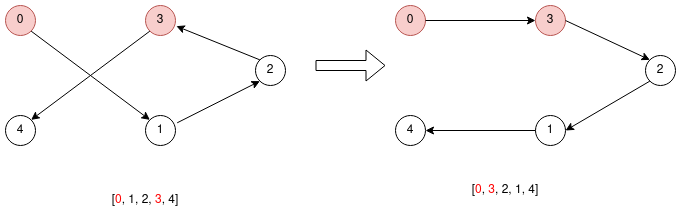
\includegraphics[width=\textwidth]{chapters/literature/img/2exdrawio.png}
      \caption{Przykład procedury 2-exchange}
      \label{fig:2exchange}
\end{figure}
